\cotefile{29}
\scanpage{63}\mspage{3.}
d'application \unsure{ds|dans} le théorème de spécialisation \deleted{\unsure{du groupe|des groupes}} des variétés \unsure{lisses} ---

Lorsque $X$ n'est pas \unsure{normale|normal}, on utilise la descente ---- À détailler.

% Sketch in the left margin of the preceding lines.
\figure{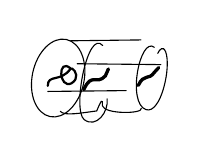
\begin{tikzpicture}[x=.55cm,y=.55cm,line cap=round]
\draw[rotate around={-12:(.62,.05)}] (.62,.05) ellipse (.60 and .91);
\draw[thin] (1.65,.80) .. controls (1.30,1.20) and (.94,-.68) .. (1.22,-.91) .. controls (1.50,-1.12) and (1.79,-.73) .. (1.75,-.43);
\draw (2.84,.76) .. controls (2.51,1.02) and (2.20,-.53) .. (2.65,-.68) .. controls (2.99,-.79) and (3.24,.31) .. (3.10,.66) .. controls (3.04,.80) and (2.96,.71) .. (2.92,.62);
\draw (.91,.91)--(2.53,.93) (1.06,.38)--(2.99,.36) (.38,-.26)--(2.19,-.24);
\draw (.67,-.72) .. controls (.77,-.83) and (1.12,-.76) .. (1.51,-.71) .. controls (1.61,-.47) and (1.65,-.40) .. (1.64,-.59) .. controls (1.69,-.79) and (2.58,-.78) .. (2.54,-.65);
\draw[thick] (.38,-.13).. controls (.38,.15) and (.68,-.06) .. (.91,.27) .. controls (.60,.54) and (.63,-.22) .. (.93,-.07) .. controls (1.11,.04) and (1.03,.22) .. (.94,.27);
\draw[very thick] (1.21,-.22).. controls (1.40,.20) and (1.50,-.13) .. (1.71,.10) --(1.78,.26);
\draw[very thick] (2.47,-.12).. controls (2.60,.16) and (2.71,-.01) .. (2.84,.18)--(2.94,.29);
\end{tikzpicture}}

% Vertical emphasis stroke beside this corollary.
\uline{Corollaire} \deleted{\illegible{1}} Soit $U$ de type fini sur $k$, $Y$
\deleted{\unsure{de type fini sur}} \unsure{propre.|propr.} sur $k$ \inserted{$y\in Y$} $R$ un revêt
étale \inserted{\unsure{gal|soit}} de $U\times_k Y$, de \unsure{groupe|gp} \unsure{$\Gamma$|$\pi$} premier \unsure{à $p$}.
\deleted{\unsure{Alors $U$}} Si $R_y$ est un rev. fini trivial,
Alors $R$ est, au dessus d'un voisinage \deleted{\unsure{de $U\times_k y$}}
$y$, l'image inverse d'un rev. \unsure{étale} d'un tel voisinage.

% Two vertical emphasis strokes beside this corollary.
\uline{Cor.} Soient $X'$, $X''$ propres sur $k$,
$Z'$ ($Z''$) des parties fermées, \deleted{\unsure{alors}} considérons
\deleted{\unsure{$Z$}} $X=\unsure{{\alpha}'|X'}\times{\alpha}''$, $Z=Z'\times X''\cup X'\times Z''$, enfin considérons
les groupes $\pi_1^t(X';Z',x')$, $\pi_1^t(X'';Z'';x'')$ et
$\pi_1^t(X\deleted{\unsure{'\times X''}};Z,x)$, \deleted{Alors} \unsure{soit|notés} $\pi,\pi';\pi''$. Alors
\[
\deleted{\pi_1^t(X)}\;\pi\longrightarrow\pi'\times\pi''
\]
est un \uline{isomorphisme}.

% Two vertical emphasis strokes beside this corollary.
\uline{Cor.} Soient $X$ $Y$ de type fini sur $k$. Considérons
$\pi'_1(X)$ \unsure{et,|et} $\pi'_1(Y)$, \inserted{$\pi'_1(X\times Y)$} [rev. étls premiers à la car].
Alors $\pi'_1(X\times Y)\simeq\pi'_1(X)\times\pi'_1(Y)$.
% archive sheet number: 62
